%
% Einleitung zum Skript über lineare Algebra
%
% (c) 2012 Prof Dr Andreas Mueller, Hochschule Rapperswil
%
\chapter*{Einleitung}

Die lineare Algebra stellt sich als Grundlage einer grossen
Zahl von Theorien heraus.
Aufgabe dieser Vorlesung ist, die
Grundlagen dieser Theorie sowie die wichtigsten Anwendungsthemen
zu vermitteln.
Um die Darstellung der Theorie nicht zu stark zu unterbrechen,
werden grösser Anwendungen in separaten Abschnitten am Ende
jedes Kapitels beschrieben.

\section*{Behandelte Themen}
\subsection*{Kapitel 1: Lineare Gleichungssysteme}
Die Lineare Algebra beschäftigt sich zunächst mit der Lösung linearer
Gleichungen.
Dazu werden im ersten Kapitel einige Methoden bereitgestellt,
und es wird diskutiert, unter welchen Voraussetzungen ein
Gleichungssystem keine, genau eine oder unendlich viele
Lösungen hat.
Die Techniken motivieren auch einen neuen Kalkül, die Matrizenrechnung,
welcher das Rechnen mit Zahlen und Vektoren, das vielen
Studierenden bereits bekannt ist, auf beliebige Dimensionen erweitert,
und zudem ein Produkt einführt.

\subsection*{Kapitel 2: Determinanten}
Für Gleichungssysteme mit gleich vielen Gleichungen wie Unbekannten
kann man ein Art Kennzahl finden, welche direkt Aussagen kann,
ob ein Gleichungssystem eine eindeutige Lösung hat.
Erstaunlicherweise ist die so definierte Grösse, die Determinante,
noch viel universeller.
Man kann damit auch direkt ein Gleichungssystem lösen, oder
die inverse Matrix berechnen.
Ausserdem lässt sich die Determinante zur Flächen- und Volumenberechnung
verwenden, und man kann damit das Vektorprodukt definieren.

\subsection*{Kapitel 3: Vektorgeometrie}
Die abstrakte Sprache der Vektoren kann auf die Geometrie angewendet
werden.
Lösungen geometrischer Aufgaben werden damit berechenbar,
meistens als Lösungen lineare Gleichungssysteme.

\subsection*{Kapitel 4: Lineare Räume}
Die Lineare Algebra ist besonders gut auf spezielle
Teilmengen des Raumes adaptiert, nämlich Geraden,
Ebenen oder höherdimensionale Analoga.

\subsection*{Kapitel 5: Matrixzerlegungen}
Der Gauss-Algorithmus aus Kapitel~1 kann auch als eine
Zerlegung einer Matrix in zwei Dreiecksmatrizen formuliert werden.
Es lassen sich aber auch andere Zerlegungen finden, die je
nach Anwendungsfall geeigneter sind.

\subsection*{Kapitel 6: Eigenwerte und Eigenvektoren}
Das wahrscheinlich wichtigste Problem der lineare Algebra
ist das Eigenwertproblem.
Dieses Kapitel beschreibt das Problem und die Lösung mit Hilfe
des charakteristischen Polynoms.
In einem eigenen Abschnitt werden ausserdem numerische Algorithmen
beschrieben, die Eigenwerte und Eigenvektoren auch für grössere
Matrizen finden können, für welche das charakteristische 
Polynom keinen praktikablen Lösungsweg darstellt.

\section*{Anwendungen}
Jedes Kapitel enthält am Ende auch einen Abschnitt mit grösseren
Anwendungen der Theorie des Kapitels.

\subsection*{Die Kirchhoffschen Gesetze}
Die Kirchhoffschen Gesetze erlauben die Ströme in einem Netzwerk
zu berechnen.
Dieses Problem wurde ursprünglich von Gustav Robert Kirchhoff
formuliert und gelöst, aber als Nebenresultate seiner Theorie
entstand auch eine ganze Menge von Resultaten über Netzwerke,
zum Beispiel zeigt sich, wie man mit Hilfe von Determinanten
die Zahl der möglichen Spannbäume eines Graphen zählen kann.

\subsection*{Kurvenanpassung}
Die Methode der kleinsten Quadrate liefert auch eine Methode,
mit der man zu einer Menge von Messwerten eine bestmöglich passende
Funktion finden kann.

\subsection*{Wavelets}
Die Orthogonalisierungsmethode erlaubt eine Menge von
Basisfunktionen zu finden, nach denen man eine gesamplete Funktion
besonders effizient entwickeln kann, und deren Weiterentwicklung
zu den Wavelets von grosser praktischer Bedeutung ist.

\subsection*{Google Pagerank}
Suchmaschinen im Internet müssen aus einer potentiell sehr grossen Zahl
von Suchresultaten die treffendsten als erste liefern.
Die einzige Quelle zur Bewertung der Resultate kann nur
das Internet selbst sein.

\section*{Die Karte der linearen Algebra}
Die Karte der linearen Algebra auf der folgenden Seite zeigt ein
paar Begriffe, die in den nachfolgenden Kapiteln erklärt werden.
Der Leser wird aufgefordert, bei Gelegenheit zu dieser Karte
zurückzukommen und zu versuchen, ob er den dargestellten
Zusammenhängen einen Sinn geben kann.

\begin{landscape}
\begin{center}
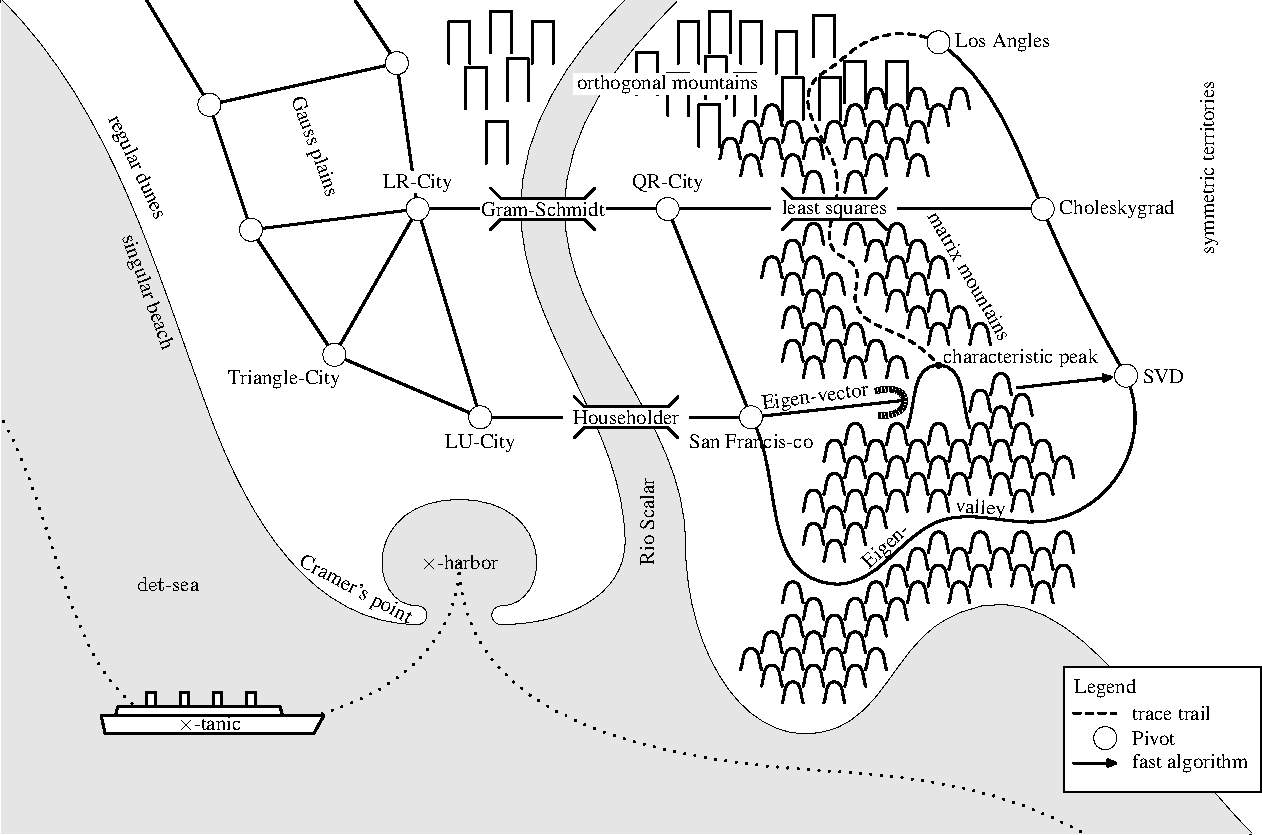
\includegraphics[width=0.95\hsize]{images/linalgmap-1}
\end{center}
\end{landscape}
